\documentclass[journal,12pt,twocolumn]{IEEEtran}

\usepackage{setspace}
\usepackage{gensymb}
\singlespacing
\usepackage[cmex10]{amsmath}

\usepackage{amsthm}

\usepackage{mathrsfs}
\usepackage{txfonts}
\usepackage{stfloats}
\usepackage{bm}
\usepackage{cite}
\usepackage{cases}
\usepackage{subfig}

\usepackage{longtable}
\usepackage{multirow}

\usepackage{enumitem}
\usepackage{mathtools}
\usepackage{steinmetz}
\usepackage{tikz}
\usepackage{circuitikz}
\usepackage{verbatim}
\usepackage{tfrupee}
\usepackage[breaklinks=true]{hyperref}
\usepackage{graphicx}
\usepackage{tkz-euclide}

\usetikzlibrary{calc,math}
\usepackage{listings}
    \usepackage{color}                                            %%
    \usepackage{array}                                            %%
    \usepackage{longtable}                                        %%
    \usepackage{calc}                                             %%
    \usepackage{multirow}                                         %%
    \usepackage{hhline}                                           %%
    \usepackage{ifthen}                                           %%
    \usepackage{lscape}     
\usepackage{multicol}
\usepackage{chngcntr}

\DeclareMathOperator*{\Res}{Res}

\renewcommand\thesection{\arabic{section}}
\renewcommand\thesubsection{\thesection.\arabic{subsection}}
\renewcommand\thesubsubsection{\thesubsection.\arabic{subsubsection}}

\renewcommand\thesectiondis{\arabic{section}}
\renewcommand\thesubsectiondis{\thesectiondis.\arabic{subsection}}
\renewcommand\thesubsubsectiondis{\thesubsectiondis.\arabic{subsubsection}}


\hyphenation{op-tical net-works semi-conduc-tor}
\def\inputGnumericTable{}                                 %%

\lstset{
%language=C,
frame=single, 
breaklines=true,
columns=fullflexible
}
\begin{document}


\newtheorem{theorem}{Theorem}[section]
\newtheorem{problem}{Problem}
\newtheorem{proposition}{Proposition}[section]
\newtheorem{lemma}{Lemma}[section]
\newtheorem{corollary}[theorem]{Corollary}
\newtheorem{example}{Example}[section]
\newtheorem{definition}[problem]{Definition}

\newcommand{\BEQA}{\begin{eqnarray}}
\newcommand{\EEQA}{\end{eqnarray}}
\newcommand{\define}{\stackrel{\triangle}{=}}
\bibliographystyle{IEEEtran}
\raggedbottom

\providecommand{\mbf}{\mathbf}
\providecommand{\pr}[1]{\ensuremath{\Pr\left(#1\right)}}
\providecommand{\qfunc}[1]{\ensuremath{Q\left(#1\right)}}
\providecommand{\sbrak}[1]{\ensuremath{{}\left[#1\right]}}
\providecommand{\lsbrak}[1]{\ensuremath{{}\left[#1\right.}}
\providecommand{\rsbrak}[1]{\ensuremath{{}\left.#1\right]}}
\providecommand{\brak}[1]{\ensuremath{\left(#1\right)}}
\providecommand{\lbrak}[1]{\ensuremath{\left(#1\right.}}
\providecommand{\rbrak}[1]{\ensuremath{\left.#1\right)}}
\providecommand{\cbrak}[1]{\ensuremath{\left\{#1\right\}}}
\providecommand{\lcbrak}[1]{\ensuremath{\left\{#1\right.}}
\providecommand{\rcbrak}[1]{\ensuremath{\left.#1\right\}}}
\theoremstyle{remark}
\newtheorem{rem}{Remark}
\newcommand{\sgn}{\mathop{\mathrm{sgn}}}
\providecommand{\abs}[1]{\left\vert#1\right\vert}
\providecommand{\res}[1]{\Res\displaylimits_{#1}} 
\providecommand{\norm}[1]{\left\lVert#1\right\rVert}
%\providecommand{\norm}[1]{\lVert#1\rVert}
\providecommand{\mtx}[1]{\mathbf{#1}}
\providecommand{\mean}[1]{E\left[ #1 \right]}
\providecommand{\fourier}{\overset{\mathcal{F}}{ \rightleftharpoons}}
%\providecommand{\hilbert}{\overset{\mathcal{H}}{ \rightleftharpoons}}
\providecommand{\system}{\overset{\mathcal{H}}{ \longleftrightarrow}}
	%\newcommand{\solution}[2]{\textbf{Solution:}{#1}}
\newcommand{\solution}{\noindent \textbf{Solution: }}
\newcommand{\cosec}{\,\text{cosec}\,}
\providecommand{\dec}[2]{\ensuremath{\overset{#1}{\underset{#2}{\gtrless}}}}
\newcommand{\myvec}[1]{\ensuremath{\begin{pmatrix}#1\end{pmatrix}}}
\newcommand{\mydet}[1]{\ensuremath{\begin{vmatrix}#1\end{vmatrix}}}
\numberwithin{equation}{subsection}

\makeatletter
\@addtoreset{figure}{problem}
\makeatother
\let\StandardTheFigure\thefigure
\let\vec\mathbf

\renewcommand{\thefigure}{\theproblem}

\def\putbox#1#2#3{\makebox[0in][l]{\makebox[#1][l]{}\raisebox{\baselineskip}[0in][0in]{\raisebox{#2}[0in][0in]{#3}}}}
     \def\rightbox#1{\makebox[0in][r]{#1}}
     \def\centbox#1{\makebox[0in]{#1}}
     \def\topbox#1{\raisebox{-\baselineskip}[0in][0in]{#1}}
     \def\midbox#1{\raisebox{-0.5\baselineskip}[0in][0in]{#1}}
\vspace{3cm}
\title{Assignment 5}
\author{Sachinkumar Dubey - EE20MTECH11009}
\maketitle
\newpage
\bigskip
\renewcommand{\thefigure}{\theenumi}
\renewcommand{\thetable}{\theenumi}
Download all python codes from 
\begin{lstlisting}
https://github.com/sachinomdubey/Matrix-theory/Assignment5/codes
\end{lstlisting}
%
and latex-tikz codes from 
%
\begin{lstlisting}
https://github.com/sachinomdubey/Matrix-theory/Assignment5
\end{lstlisting}
\subsection{Problem}
(Geolin 1.9) $AB$ is a line-segment. $P$ and $Q$ are points on opposite sides of $AB$ such that each of them is equidistant from the points $A$ and $B$. Show that the line $PQ $ is the perpendicular bisector of $AB$.\\
\begin{figure}[h!]
\centering
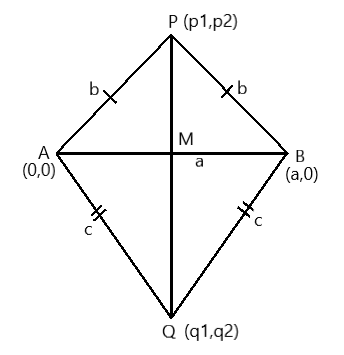
\includegraphics[width=7cm, height=7cm]{Figure_51}
\caption{}
\label{Fig4}
\end{figure}
\\
\subsection{Explanation}
In order to prove that line $PQ $ is the perpendicular bisector of $AB$, two conditions need to be met:
\begin{enumerate}
        \item $PQ \perp AB $
    \item $AM$=$BM$
\end{enumerate}
These conditions can be proved as follow:
\subsection{Solution}
\noindent It is given that the points $\vec{P}$ and $\vec{Q}$  are equidistant from the points $\vec{A}$ and $\vec{B}$. Thus we can write:
\begin{align}
    \norm{\vec{P}-\vec{A}}=\norm{\vec{P}-\vec{B}} \label{eq2.2}\\
    \norm{\vec{Q}-\vec{A}}=\norm{\vec{Q}-\vec{B}} \label{eq2.3}
\end{align}
Squaring both sides of equations \ref{eq2.2} and expanding further, we can write:
\begin{align}
    \brak{\vec{P}-\vec{A}}^T\brak{\vec{P}-\vec{A}}=\brak{\vec{P}-\vec{B}}^T\brak{\vec{P}-\vec{B}} \\
    \vec{P}^T\vec{P}-\vec{P}^T\vec{A}-\vec{A}^T\vec{P}+\vec{A}^T\vec{A}= \nonumber \\ 
     \vec{P}^T\vec{P}-\vec{P}^T\vec{B}-\vec{B}^T\vec{P}+\vec{B}^T\vec{B} \\
     \therefore \vec{A}^T\vec{A}-\vec{B}^T\vec{B}=-2\vec{P}^T\vec{B}+2\vec{P}^T\vec{A}\label{eq3.5}
\end{align}
Similarly, Squaring both sides of equations \ref{eq2.3} and expanding further, we can write:
\begin{align}
    \brak{\vec{Q}-\vec{A}}^T\brak{\vec{Q}-\vec{A}}=\brak{\vec{Q}-\vec{B}}^T\brak{\vec{Q}-\vec{B}} \\
    \vec{Q}^T\vec{Q}-\vec{Q}^T\vec{A}-\vec{A}^T\vec{Q}+\vec{A}^T\vec{A}= \nonumber \\ 
     \vec{Q}^T\vec{Q}-\vec{Q}^T\vec{B}-\vec{B}^T\vec{Q}+\vec{B}^T\vec{B} \\
     \therefore \vec{A}^T\vec{A}-\vec{B}^T\vec{B}=-2\vec{Q}^T\vec{B}+2\vec{Q}^T\vec{A}\label{eq3.8}
\end{align}
From equations \ref{eq3.5} and \ref{eq3.8}, we can write:
\begin{align}
    2\vec{P}^T\brak{\vec{A}-\vec{B}}=2\vec{Q}^T\brak{\vec{A}-\vec{B}}\\
    \vec{P}^T\brak{\vec{A}-\vec{B}}-\vec{Q}^T\brak{\vec{A}-\vec{B}}=0\\
    \brak{\vec{P}-\vec{Q}}^T\brak{\vec{A}-\vec{B}}=0
\end{align}
Thus, Segment $PQ$ is perpendicular to segment $AB$ ($PQ \perp AB$).\\ \\
From the figure, equations \ref{eq2.2} can also be written as:
\begin{align}
    \norm{\brak{\vec{P}-\vec{M}}+\brak{\vec{M}-\vec{A}}}=\norm{\brak{\vec{P}-\vec{M}}+\brak{\vec{M}-\vec{B}}}
\end{align}
Squaring and expanding both the sides, we get:
\begin{align}
\brak{\brak{\vec{P}-\vec{M}}+\brak{\vec{M}-\vec{A}}}^T\brak{\brak{\vec{P}-\vec{M}}+\brak{\vec{M}-\vec{A}}} = \nonumber \\
\brak{\brak{\vec{P}-\vec{M}}+\brak{\vec{M}-\vec{B}}}^T\brak{\brak{\vec{P}-\vec{M}}+\brak{\vec{M}-\vec{B}}}
\end{align}
\begin{align}
\brak{\vec{P}-\vec{M}}^T\brak{\vec{P}-\vec{M}}+\brak{\vec{P}-\vec{M}}^T\brak{\vec{M}-\vec{A}}+ \nonumber \\\brak{\vec{M}-\vec{A}}^T\brak{\vec{P}-\vec{M}}+\brak{\vec{M}-\vec{A}}^T\brak{\vec{M}-\vec{A}} = \nonumber \\
\brak{\vec{P}-\vec{M}}^T\brak{\vec{P}-\vec{M}}+\brak{\vec{P}-\vec{M}}^T\brak{\vec{M}-\vec{B}}+ \nonumber \\\brak{\vec{M}-\vec{B}}^T\brak{\vec{P}-\vec{M}}+\brak{\vec{M}-\vec{B}}^T\brak{\vec{M}-\vec{B}}\\
\norm{\brak{\vec{M}-\vec{A}}}^2+2\brak{\vec{M}-\vec{A}}^T\brak{\vec{P}-\vec{M}} = \nonumber \\
\norm{\brak{\vec{M}-\vec{B}}}^2+2\brak{\vec{M}-\vec{B}}^T\brak{\vec{P}-\vec{M}} \label{eq3.15}
\end{align}
Since, $PQ\perp AB$. Hence, we can write:
\begin{align}
\brak{\vec{M}-\vec{A}}^T\brak{\vec{P}-\vec{M}}=\brak{\vec{M}-\vec{B}}^T\brak{\vec{P}-\vec{M}}=0 \label{eq3.16}
\end{align}
From equation \ref{eq3.15} and \ref{eq3.16}, we get:
\begin{align}
    \norm{\brak{\vec{M}-\vec{A}}}=\norm{\brak{\vec{M}-\vec{B}}}
\end{align}
Thus, $M$ is the midpoint of segment $AB$ ($AM=BM$).
Thus, Segment $PQ$ is perpendicular bisector of segment $AB$.
\end{document}